\documentclass[10pt]{beamer}

\usetheme[progressbar=frametitle]{metropolis}
\usepackage{appendixnumberbeamer}

\setbeamertemplate{bibliography item}[text]

\setbeamerfont{bibliography item}{size=\footnotesize}
\setbeamerfont{bibliography entry author}{size=\footnotesize}
\setbeamerfont{bibliography entry title}{size=\footnotesize}
\setbeamerfont{bibliography entry location}{size=\footnotesize}
\setbeamerfont{bibliography entry note}{size=\footnotesize}

\usepackage{array,booktabs}
\usepackage[scale=2]{ccicons}
\usepackage{multicol}
\usepackage{mathtools}
\usepackage{array}

\usepackage{pgfplots}
\usepgfplotslibrary{dateplot}

\usepackage{xspace}

\usepackage{tikz}

\newcommand{\themename}{\textbf{\textsc{metropolis}}\xspace}
\let\oldfootnotesize\footnotesize
\renewcommand*{\footnotesize}{\oldfootnotesize\tiny}
\let\oldabs\abs
\def\abs{\@ifstar{\oldabs}{\oldabs*}}


\title{My past, present and potential future of releasing software with my publications}
\author{Andrew Moore}
\date{\today}
\institute{School of Computing and Communications, Lancaster University.}
\titlegraphic{\hfill
\includegraphics[height=1.5cm]{ucrel_logo_2016.png}}

\begin{document}

\maketitle

\begin{frame}{Past}
\begin{block}{SemEval publication on predicting sentiment in financial news headlines\cite{fin_sem}}
\begin{center}
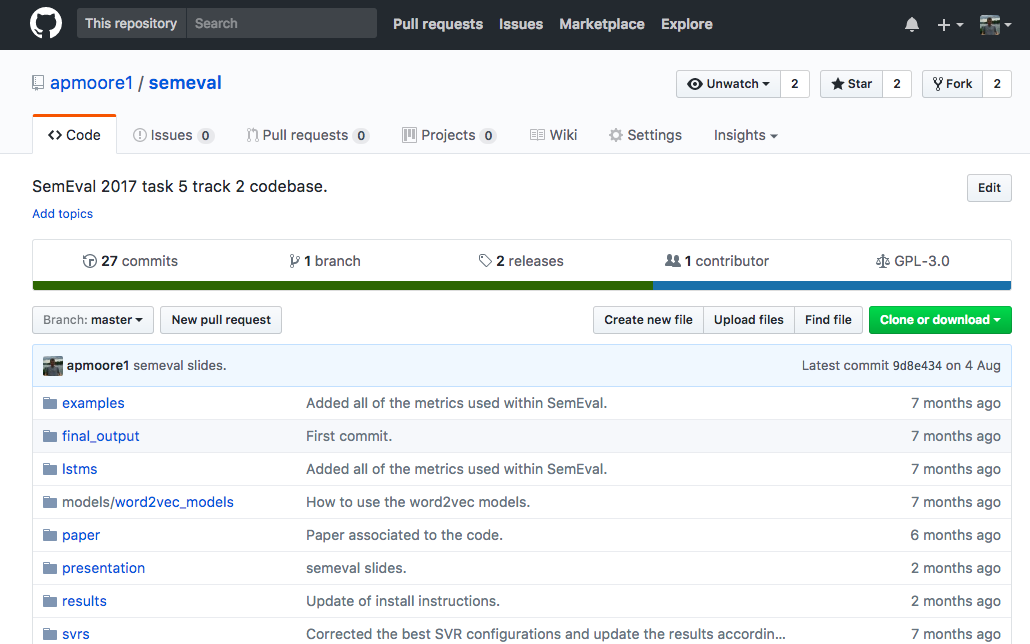
\includegraphics[scale=0.25]{semeval.png}
\end{center}
\end{block}
\end{frame}

\begin{frame}{How people can find the code}
\begin{enumerate}
\item Link in the paper.
\item Via the research directory
\end{enumerate}
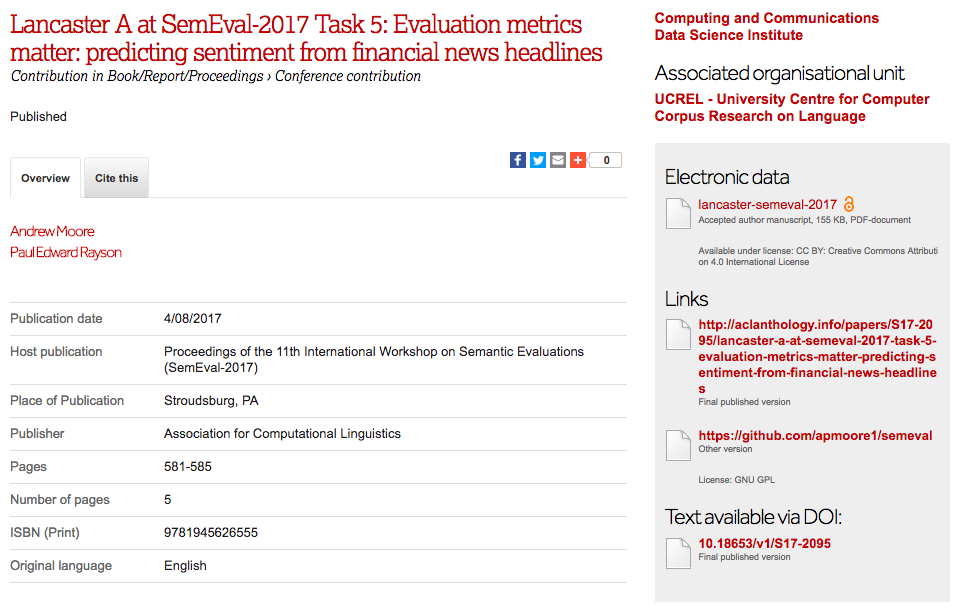
\includegraphics[scale=0.25]{publication_code.png}
\end{frame}

\begin{frame}{Present}
The problems that I found from my past:
\begin{enumerate}
\item The code does not prove what I have done has been implemented correctly.
\item The code lacks detailed documentation.
\item The code could be easier to find.
\end{enumerate}
My solutions to these problems:
\begin{enumerate}
\item Create test e.g. unit test.
\item Create detailed documentation like readthedocs.
\item My profile on the research directory to include software tab.
\end{enumerate}
\end{frame}

\begin{frame}{readthedocs example}
\begin{block}{esig python package\footnote{\url{http://esig.readthedocs.io/en/latest/}}}
\begin{center}
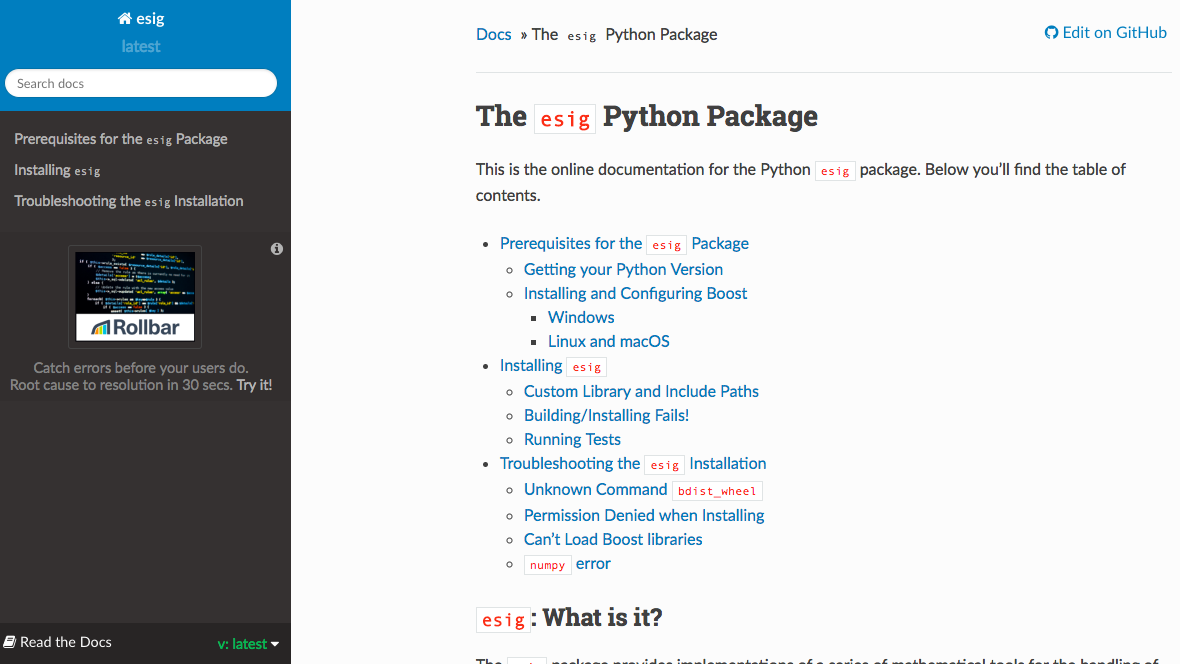
\includegraphics[scale=0.25]{esig.png}
\end{center}
\end{block}

\end{frame}

\begin{frame}{Research directory example}
\centering
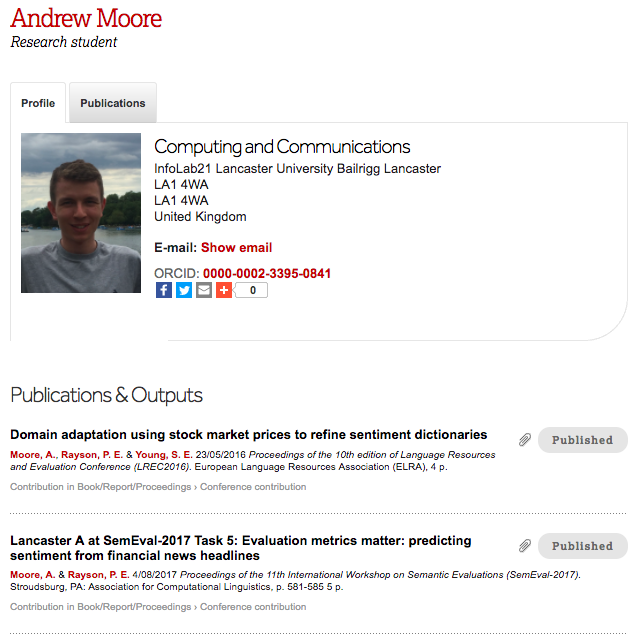
\includegraphics[scale=0.3]{publication.png}
\end{frame}

\begin{frame}{Future}
What I would like to see more of:
\begin{enumerate}
\item More researchers releasing their code.
\end{enumerate}
The reasons I hear why researchers don't release their code:
\begin{enumerate}
\item I don't have the time.
\item I don't like the way the code is at the moment.
\item It is my code/ I don't want to.
\end{enumerate}
\end{frame}

\begin{frame}{My answers/solutions}
\begin{enumerate}
\item Releasing the code no matter what it looks like is better than not.
\item When it is released others might help you.
\item Research Software Engineers (RSE)
\item More time/money
\end{enumerate}
\end{frame}

\begin{frame}{Spending more time/money is better}
Reasons for RSE and more time on making the code easier to use:
\begin{enumerate}
\item Higher impact for your research
\item Allow other researchers to perform their job faster
\end{enumerate}
\begin{block}{Example}
Stanford CoreNLP\cite{corenlp}\footnote{\url{https://stanfordnlp.github.io/CoreNLP/}} has:
\begin{enumerate}
\item 1711 citations
\item 3771 stars and been forked 1409 times on Github
\end{enumerate}, 
\end{block}
\end{frame}



\begin{frame}[plain]
\begin{center}
\huge Questions?
\end{center}
\centering
Andrew Moore
\\
@apmoore94
\\
Slides: \url{https://github.com/apmoore1/software-as-data}
\end{frame}


\begin{frame}[allowframebreaks]{References}
  \bibliography{demo}
  \bibliographystyle{abbrv}
\end{frame}

\end{document}
